\section{Ricerca}

La \emph{ricerca}, in un sito con una tale mole di dati, è assolutamente essenziale che sia 
presente, e ancora più importante, che funzioni bene.

Andiamo ad analizzarla nel dettaglio, vedendo prima un paio di immagini.

\begin{figure}[hbt]
    \centering
    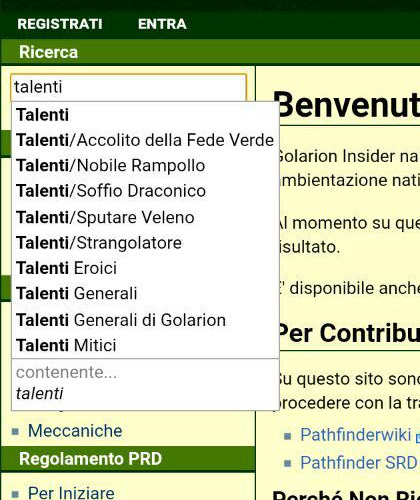
\includegraphics[width=5cm]{img/ricerca1.jpg}
    \caption{Suggerimenti di ricerca nello strumento in alto a sinistra.}
\end{figure}

\begin{figure}[hbt]
    \centering
    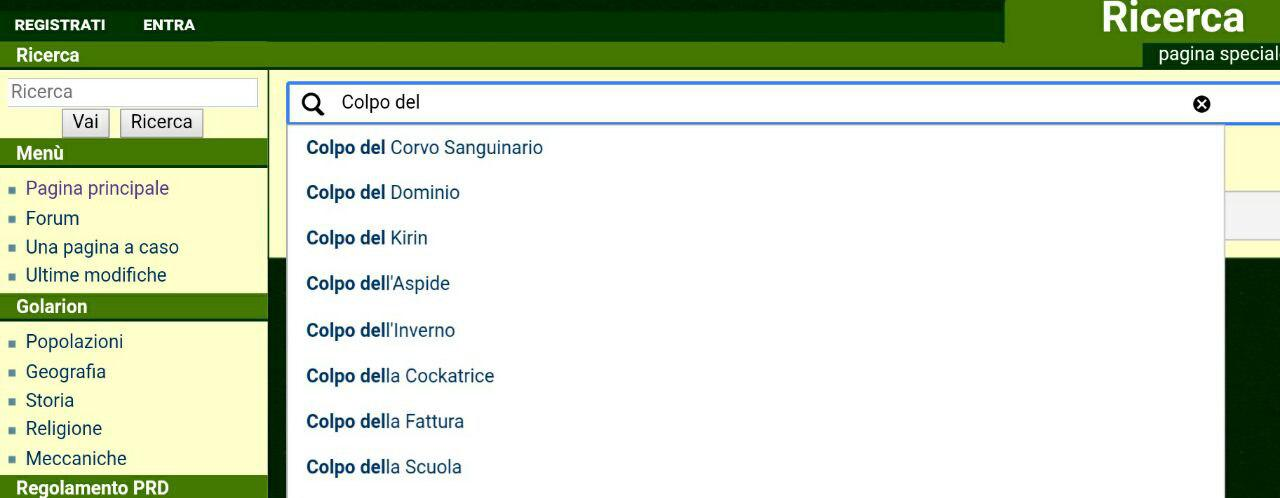
\includegraphics[width=\textwidth]{img/ricerca2.jpg}
    \caption{Suggerimenti di ricerca nel tool di ricerca alternativo.}
\end{figure}

Lo strumento di ricerca semplice è ben curato, e i suggerimenti sono un ottimo aiuto per mettere l'utente a proprio agio.
Un problema rilevato durante l'analisi è che se esiste una pagina con il nome della keyword/delle keywords inserite,
si viene automaticamente reindirizzati a quella pagina, e non è sempre il comportamento atteso. A volte fa risparmiare dei click,
mentre altre rischia di causare stress nel visitatore. In ogni caso, non si viene mai reindirizzati in una nuova scheda, e questo
è positivo, poichè mantiene la cronologia e permette di sfruttare il tasto \emph{back}, molto prezioso per l'utente.\par
\smallskip
Vediamo un caso di ricerca per parole chiave, nel fortunato caso in cui non si venga automaticamente indirizzati in
una pagina (è stata cercata la parola \texttt{Arcana}).

\begin{figure}[hbt]
    \centering
    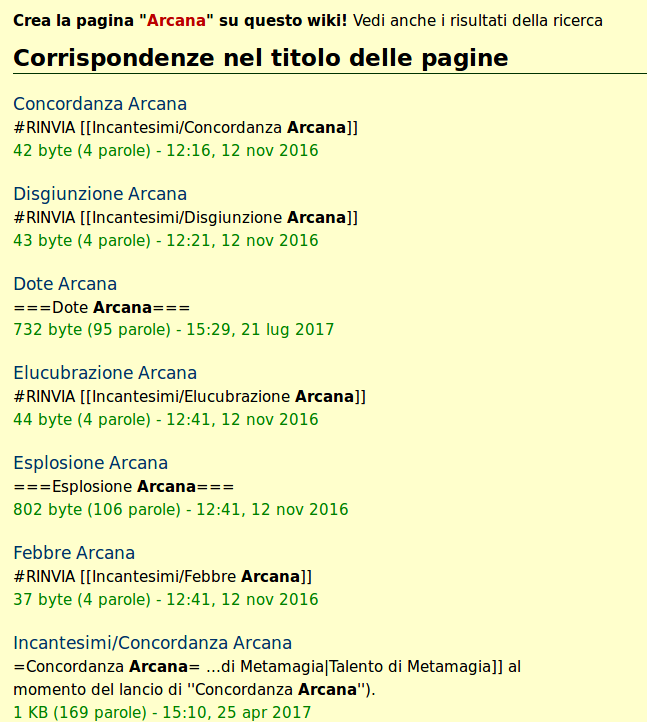
\includegraphics[width=0.5\textwidth]{img/ricerca4.png} 
    \caption{Ricerca per parole chiave con corrispondenza nei titoli.}
\end{figure}

\begin{figure}[!hbt]
    \centering
    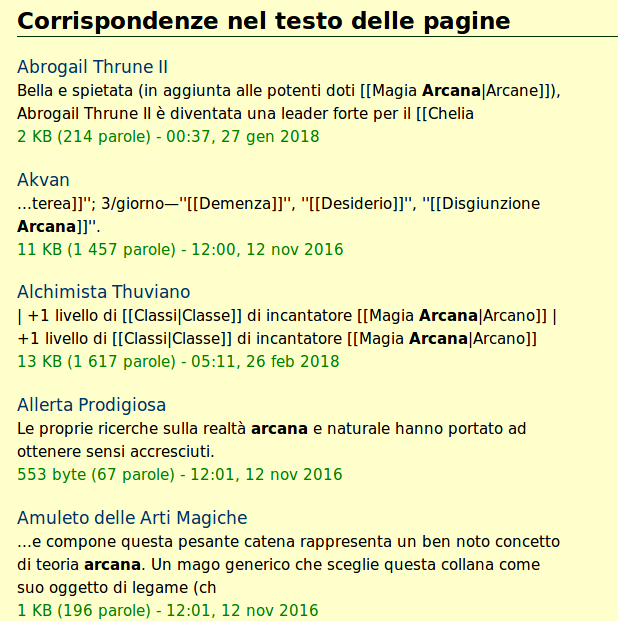
\includegraphics[width=0.5\textwidth]{img/ricerca5.png} 
    \caption{Ricerca per parole chiave con corrispondenza nel testo delle pagine.}
\end{figure} 

Scrollando la pagina, otterremo due risultati:
\begin{itemize}
    \item \emph{Corrispondenze nel titolo delle pagine}: in questa sezione avremo i risultati in cui la parola chiave (o le parole chiave)
    appare nel titolo;
    \item \emph{Corrispondenza nel testo delle pagine}: qui, invece, i risultati in cui la parola chiave è nel testo.
\end{itemize}

Una suddivisione del genere può aiutare, ma durante l'utilizzo del sito sono state rare le volte in cui personalmente 
è tornata utile.

\subsection{Posizionamento}

La scelta del \emph{posizionamento} (in alto a sinistra, sotto al logo) del tool di ricerca è anche qui azzeccata. 
Facile da notare, e da raggiungere con il mouse.

\subsection{Ricerca avanzata}

Vediamo come si presenta la ricerca avanzata.

\begin{figure}[hbt]
    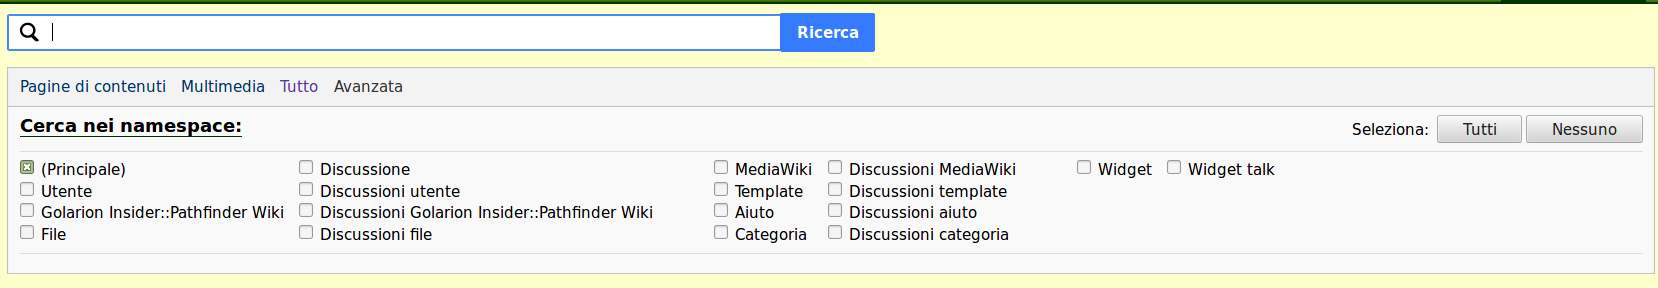
\includegraphics[width=\textwidth]{img/ricerca3.png}
    \caption{Ricerca avanzata.}
\end{figure}

Non si presenta per niente bene. Avere delle opzioni del genere, è totalmente inutile e non da alcun aiuto, anzi, 
rischia di confondere. Questo perchè non c'è assolutamente nulla nelle varie sotto-sezioni, quali ad esempio
\texttt{Discussioni MediaWiki}, o \texttt{Discussioni template}.\par
Uno strumento di ricerca avanzato ben implementato, ti permetterebbe di cercare delle parole chiave \emph{solo}
in determinate categorie: ad esempio, vorrei cercare solamente tra gli \texttt{Oggetti Magici} quelli che nel nome
o nella loro descrizione contengono la parola \texttt{Attacco di Opportunità}. Questo non è possibile alla versione
del sito attuale, e la cosa ironica è che in molti casi non è nemmeno possibile sfruttare la ricerca semplice per tale
scopo, poichè cercando un insieme di parole chiave che ha una pagina dedicata si viene reindirizzati automaticamente alla pagina
con tale nome!